% Built on the official ISBI 2027 template (spconf.sty / IEEEbib.bst),
% from ISBI_template-master.zip, biomedicalimaging.org/2027/contributors/papers/
\documentclass{article}
\usepackage{spconf,amsmath,graphicx}
\usepackage{times}
\usepackage[T1]{fontenc}
\usepackage[utf8]{inputenc}
\usepackage{amssymb}
\usepackage{tikz}
\usetikzlibrary{arrows.meta}
\usepackage{booktabs}
\usepackage{enumitem}
\setlist{nosep, leftmargin=14pt}

\newcommand{\shiftgap}{\ensuremath{G}}
\newcommand{\lrand}{\ensuremath{L_{\text{rand}}}}
\newcommand{\lsite}{\ensuremath{L_{\text{site}}}}

\title{Site-robust ensemble classification of DaT-SPECT scans under severe scanner heterogeneity}

\name{Harshdip Saha}
\address{Independent Researcher\\harshdipsaha@gmail.com}

\begin{document}
\maketitle

\begin{abstract}
Automated dopamine-transporter (DaT) SPECT classification looks solved: prior work reports 96--99\% accuracy, almost entirely on the single-center, pre-registered PPMI cohort. We report a case study on a new, unpublished, ten-hospital DaT-SPECT dataset (DrivenData Competition \#311) whose sites differ in native voxel spacing, volume shape, and count-rate regime, with no pre-registration and an undisclosed hidden-test site mix. We describe a five-pillar ensemble (hemisphere-split 3D, self-supervised 3D, radiomics-feature, coronal 2.5D, and axial 2.5D arms) combined via temperature-scaled, prior-adjusted log-odds averaging. We introduce the \emph{shift gap} --- the difference between random-fold and leave-site-out out-of-fold log loss --- as a diagnostic for cross-site generalization requiring no hidden-test access. On our current ensemble this gap is 0.005--0.008, smaller than the 0.018--0.021 nested-to-public gap observed on two real submissions to date; we report this discrepancy honestly rather than as solved. Results are interim (competition closes September 16, 2026); the pipeline's best real submission ranks 44th of 450 (log loss 0.2667, AUROC 0.9536).
\end{abstract}

\begin{keywords}
DaT-SPECT, Parkinson's disease, domain generalization, ensemble learning, multi-site medical imaging
\end{keywords}

\section{Introduction}
\label{sec:intro}

More than 20{,}000 DaT scans are read each year in France, and roughly one in five involves an early-stage or atypical presentation difficult to classify confidently \cite{isbi_challenge}. The DrivenData ``DaT Parkinson's Challenge'' (\#311), organized by the French Society of Nuclear Medicine under France's France~2030 program, targets exactly this ambiguous middle ground, with the winning model slated for release into France's open health-algorithm library (BOAS).

Published DaT-SPECT classifiers cluster at 96--99\% accuracy and AUROC above 0.98 \cite{choi2017,quan2019,ensemblefusion2022}, but almost all of that work is built on PPMI: one or two centers, pre-normalized to a common template. The present dataset is structurally different --- ten hospitals, each with native voxel spacing and grid shape, no guaranteed pre-registration, and an undisclosed test-set site mix --- which is the domain-generalization problem the PPMI literature mostly avoids. Because the competition scores log loss, which punishes confident wrong answers far more than accuracy does, calibration under site shift matters as much as discrimination.

This paper contributes: (1) a five-pillar ensemble on a shared, label-blind registered frame, robust to each hospital's native acquisition geometry; (2) a log-loss-specific combiner (weighted log-odds, fitted temperature, prevalence prior mix); (3) the \emph{shift gap}, an acquisition-metadata-only diagnostic for cross-site generalization, measured here against real leaderboard behavior and found to capture only part of it; and (4) an honest interim case study, reported ahead of the competition's close.

\section{Related work}
\label{sec:related}

Automated DaT-SPECT classification is a mature line of work: 3D CNNs on MNI-normalized PPMI volumes reach 96.0--98.8\% accuracy, including one of the few genuinely independent-cohort validations in this literature \cite{choi2017}; slice-based transfer learning and multi-model fusion reach 98--98.5\% but on 1--3 selected 2D slices rather than full volumes \cite{quan2019,ensemblefusion2022}. The largest cohort with a genuine blind held-out test (1{,}017 subjects, single-center) reports a sensitivity/specificity drop from cross-validation to blind testing \cite{zhao2022}, and the only cross-scanner generalization test in this literature splits PPMI by SPECT manufacturer \cite{radiomics2022}. None of this literature reports log loss, and only two of five studies use a genuinely held-out test rather than cross-validation only --- the gap this paper's evaluation protocol targets. Temperature scaling \cite{guo2017} and deep ensembles \cite{lakshminarayanan2017} inform our combiner; the domain-generalization literature \cite{gulrajani2021} motivates the shift gap as a directly computable, acquisition-metadata-only instantiation of leave-one-domain-out validation.

\section{Data}
\label{sec:data}

The dataset comprises compressed NIfTI volumes (16-bit intensities) from ten French hospitals, with a binary label (\texttt{is\_pathologic}) from the organizing radiologists. Unlike PPMI, native shapes range from roughly $128^3$ to $142\times142\times112$ voxels and native isotropic spacing from 2.46--3.9\,mm across sites, with no pre-registration before release and hospital identity withheld for every scan. We construct a \emph{pseudo-site} fingerprint --- native voxel spacing, grid shape, and intensity regime --- as an unsupervised acquisition-site proxy for validation only. The hidden test set is mounted only inside the competition's code-execution container; its size, split, and site composition are undisclosed. Per the competition's data-sharing rules, this paper describes but does not redistribute the dataset, following the convention established for ADNI, PPMI, and UK Biobank.

\section{Methods}
\label{sec:methods}

Every input is derived from a fixed head box (192\,mm cube region, 2\,mm isotropic, centered on head center of mass), registered to a label-blind study template built only from training volumes; a per-scan fallback reverts implausible registrations to the unregistered center-of-mass frame. Uptake is expressed in reference units (normalized to a non-striatal reference region), and three consecutive 8\,mm slabs around the template's striatal plane feed the 2.5D arms.

The ensemble's five pillars are: a \textbf{hemisphere arm} (bilateral half-crop 3D encoder, right mirrored to left, preserving one-sided deficits); a \textbf{self-supervised 3D arm} (VICReg-pretrained 3D CNN); a \textbf{feature arm} (kernel classifier over 116 handcrafted radiomics descriptors, the ensemble's only non-deep-learning member); a \textbf{coronal 2.5D arm} (ConvNeXt-style); and an \textbf{axial 2.5D arm} (EfficientNetV2-style). A sixth candidate, a tri-planar 2.5D arm, was trained but excluded from the reported ensemble (Section~\ref{sec:results}). All arms use a fixed-epoch \emph{honest protocol} (no OOF-based early stopping); five random stratified folds are used for model selection, and a separate site-fold partition (holding out whole pseudo-sites) is used only to estimate cross-site generalization. Arm probabilities are combined as a weighted average of log-odds with a fitted temperature (conventionally floored at 1) and a small training-prevalence prior mix, both aimed at log-loss calibration rather than accuracy.

Let \lrand{} and \lsite{} denote out-of-fold log loss under random and leave-pseudo-site-out folds, respectively. We define the \textbf{shift gap} as
\begin{equation}
\shiftgap = \lsite - \lrand,
\label{eq:shiftgap}
\end{equation}
computable entirely from training-time acquisition metadata, without hidden-test access, in any multi-site challenge that permits an unsupervised site-fingerprint partition.

\section{Experiments and results}
\label{sec:results}

Results are interim: the competition closes September 16, 2026, and the private leaderboard has not yet been scored at time of writing (September 11, 2026). The five-pillar ensemble (not yet submitted for real scoring) achieves random-fold OOF log loss 0.2354 (equal weights) and leave-site-out OOF log loss 0.2402, a shift gap $\shiftgap \approx 0.005$--$0.008$ (Fig.~\ref{fig:shiftgap}). This ensemble scores 0.2381 on the platform's 20-scan smoke test. A separate, earlier stack from the same pipeline, submitted for real scoring, reached public log loss 0.2667 (AUROC 0.9536), ranking 44th of 450.

\begin{figure}[t]
\centering
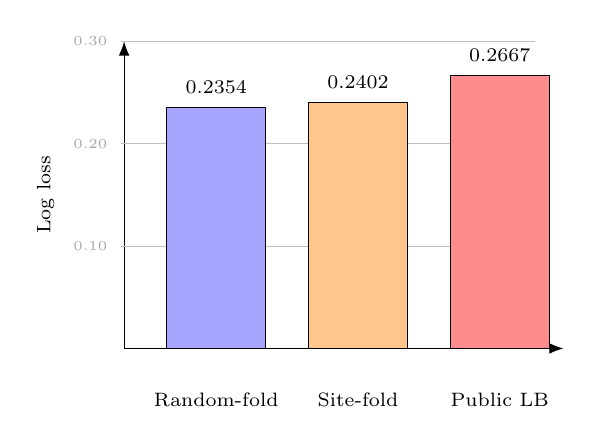
\begin{tikzpicture}[y=13cm,x=0.9cm]
\draw[-{Latex[length=1.8mm]}] (0,0) -- (0,0.30);
\node[font=\scriptsize, rotate=90, anchor=south] at (-0.85,0.15) {Log loss};
\draw[-{Latex[length=1.8mm]}] (0,0) -- (6.2,0);
\draw[gray!50] (-0.05,0.10) -- (5.8,0.10);
\node[font=\tiny, gray!70, anchor=east] at (-0.1,0.10) {0.10};
\draw[gray!50] (-0.05,0.20) -- (5.8,0.20);
\node[font=\tiny, gray!70, anchor=east] at (-0.1,0.20) {0.20};
\draw[gray!50] (-0.05,0.30) -- (5.8,0.30);
\node[font=\tiny, gray!70, anchor=east] at (-0.1,0.30) {0.30};
\draw[fill=blue!35] (0.6,0) rectangle (2.0,0.2354);
\node[font=\scriptsize] at (1.3,0.2354+0.02) {0.2354};
\node[font=\scriptsize, align=center] at (1.3,-0.05) {Random-fold};
\draw[fill=orange!45] (2.6,0) rectangle (4.0,0.2402);
\node[font=\scriptsize] at (3.3,0.2402+0.02) {0.2402};
\node[font=\scriptsize, align=center] at (3.3,-0.05) {Site-fold};
\draw[fill=red!45] (4.6,0) rectangle (6.0,0.2667);
\node[font=\scriptsize] at (5.3,0.2667+0.02) {0.2667};
\node[font=\scriptsize, align=center] at (5.3,-0.05) {Public LB};
\end{tikzpicture}
\caption{Random-fold vs.\ leave-site-out OOF log loss for the five-pillar ensemble, alongside the public leaderboard score of an earlier, differently-composed submitted stack. The shift gap ($\approx$0.005--0.008) between the first two bars is small relative to the nested-to-public gap actually observed on real submissions (0.018--0.021, Table~\ref{tab:arms}).}
\label{fig:shiftgap}
\end{figure}

Table~\ref{tab:arms} reports standalone arm performance. The tri-planar candidate was excluded from the final stack by an OOF-fitted stacker (collinear with the hemisphere arm under random folds) despite scoring the best random-fold loss of any 2.5D arm and the strongest individual smoke-test result in the project (0.2341) --- an OOF-fitted stacker that never sees site shift cannot detect that this arm's cross-site value differs from its random-fold collinearity. The feature arm, the only arm individually site-validated, shows a per-arm shift gap (site 0.3106 vs.\ random 0.2997) larger than the ensemble's. Separately, the temperature fitted on site-fold predictions falls below 1 ($T\approx0.826$); forcing the conventional $T \geq 1$ floor \emph{worsens} site-fold loss (0.2402$\to$0.2449), indicating this calibration heuristic does not transfer under site shift.

\begin{table}[t]
\centering
\small
\caption{Standalone out-of-fold arm performance (log loss / AUROC). Weight is each arm's share of the OOF-fitted five-pillar stack (a different, fitted-weight variant from the equal-weight ensemble of Fig.~\ref{fig:shiftgap}).}
\label{tab:arms}
\begin{tabular}{@{}lccc@{}}
\toprule
\textbf{Arm} & \textbf{Random} & \textbf{Site} & \textbf{Weight} \\
\midrule
Hemisphere & 0.2379 / .9658 & --- & 50.0\% \\
Self-supervised 3D & 0.2519 / .9608 & --- & 12.5\% \\
Feature (radiomics) & 0.2997 / .9455 & 0.3106 / .9410 & 12.5\% \\
Coronal 2.5D & 0.2651 / .9571 & --- & 12.5\% \\
Axial 2.5D & 0.2630 / .9576 & --- & 12.5\% \\
Tri-planar (excluded) & 0.2560 / .9603 & --- & 0.0\% \\
\bottomrule
\end{tabular}
\end{table}

\section{Discussion and conclusion}
\label{sec:discussion}

The shift gap does not fully explain the leaderboard gap it is compared against, and we report that directly rather than treating the diagnostic as sufficient: the true hidden-test site composition may be more adversarial than the training-set's own site distribution, or the pseudo-site fingerprint may under-resolve real acquisition variability that true, undisclosed hospital identity would capture. What the diagnostic does surface, concretely, are two pipeline failures invisible to random-fold-only validation: a calibration heuristic ($T\geq1$) that reverses under site shift, and a stacking decision that discards the arm best supported by real hidden-test evidence. Both matter more, we argue, than the shift gap's raw magnitude. Limitations: results are interim and pre-final; pseudo-site is an acquisition-metadata proxy, not verified hospital identity; all contributing sites are French, bounding generalization claims; and the shift gap and the historical leaderboard-gap comparison come from two different model configurations, offered as the best available evidence of this pipeline's typical behavior rather than a controlled before/after measurement.

We describe a five-pillar, site-aware ensemble for a new, restricted-access, ten-hospital DaT-SPECT dataset and introduce the shift gap as a reusable, hidden-test-free diagnostic for cross-site generalization in multi-site medical imaging challenges. A revision will report the final private-leaderboard result once the competition closes.

\section{Compliance with ethical standards}
\label{sec:ethics}

This research study was conducted retrospectively using human-subject data made available to registered competition participants by the French Society of Nuclear Medicine, Health Data Hub, and GaelO under DrivenData Competition \#311, part of France's Health Data Challenges program. The data are restricted-access (not open-access) and governed by the competition's data-use agreement, which permits analysis but prohibits redistribution. The author did not collect the data and had no role in its original ethical review, which was the responsibility of the organizing institutions.

\section{Acknowledgments}
\label{sec:ack}

No funding was received for conducting this study. The author is a participant in DrivenData Competition \#311 and may be eligible for competition prizes; no other financial or non-financial competing interests exist. AI-assisted tools (Claude, Claude Code, Anthropic) supported pipeline engineering and manuscript drafting; all reported numbers were verified by the author against the underlying experiment logs prior to submission.

\bibliographystyle{IEEEbib}
\begin{thebibliography}{00}

\bibitem{isbi_challenge} DrivenData, ``DaT Parkinson's Challenge (Competition \#311),'' French Society of Nuclear Medicine / Health Data Hub / GaelO, 2026. [Online]. Available: https://www.drivendata.org/competitions/311/dat-parkinsons-challenge/

\bibitem{choi2017} H.~Choi, S.~Ha, H.~J.~Im, S.~H.~Paek, and D.~S.~Lee, ``Refining diagnosis of Parkinson's disease with deep learning-based interpretation of dopamine transporter imaging,'' \emph{NeuroImage: Clinical}, vol.~16, pp.~586--594, 2017.

\bibitem{quan2019} T.~M.~Quan, N.~M.~Doan, M.~Le, T.~Nguyen, and V.~Q.~Ha, ``DaTscan SPECT image classification for Parkinson's disease,'' \emph{arXiv:1909.04142}, 2019.

\bibitem{ensemblefusion2022} ``An ensemble of convolutional neural network models for the diagnosis of Parkinson's disease using DaTscan images,'' \emph{Diagnostics}, vol.~12, no.~5, art.~1173, 2022.

\bibitem{zhao2022} Y.~Zhao, J.~Wu, J.~Yuan, \emph{et al.}, ``Decoding dopamine transporter imaging for differential diagnosis of parkinsonism using deep learning,'' \emph{Eur. J. Nucl. Med. Mol. Imaging}, vol.~49, pp.~2798--2811, 2022.

\bibitem{radiomics2022} ``A radiomics signature for the diagnosis of Parkinson's disease from striatal DAT-SPECT with cross-manufacturer generalization,'' \emph{Eur. J. Nucl. Med. Mol. Imaging}, vol.~49, 2022.

\bibitem{guo2017} C.~Guo, G.~Pleiss, Y.~Sun, and K.~Q.~Weinberger, ``On calibration of modern neural networks,'' in \emph{Proc. ICML}, 2017, pp.~1321--1330.

\bibitem{lakshminarayanan2017} B.~Lakshminarayanan, A.~Pritzel, and C.~Blundell, ``Simple and scalable predictive uncertainty estimation using deep ensembles,'' in \emph{Proc. NeurIPS}, vol.~30, 2017.

\bibitem{gulrajani2021} I.~Gulrajani and D.~Lopez-Paz, ``In search of lost domain generalization,'' in \emph{Proc. ICLR}, 2021.

\end{thebibliography}

\end{document}
